\chapter{Toolchain Frontend}\label{chap:offline}
The purpose of the toolchain is to support the process from specifying assertions to generating assertion smart contracts that can be invoked on-chain by the validators. As determined in \secref{sec:restrict}, the current version of the toolchain only supports the processing of assertions featuring universal quantification. The toolchain was developed in the programming language OCaml \cite{ocaml_docs} --- the code is available in a GitHub\footnote{\url{https://github.com/proglang/thesis-distributed-assertion-checking/commit/7c22038cebe44f779621d241a8ab156e105ead0c}} repository of the Chair of Programming Languages.

As an overview, \figref{fig:pipeline_frontend} depicts all stages of the processing pipeline implemented by the toolchain. The colourized stages highlight the frontend, which was designed to be as generic as possible, s.t. it can be used (or extended) to support any target blockchain. For the target-specific processing, the intermediate result of the frontend is passed to the respective backends via a public interface.

\begin{figure}[h]
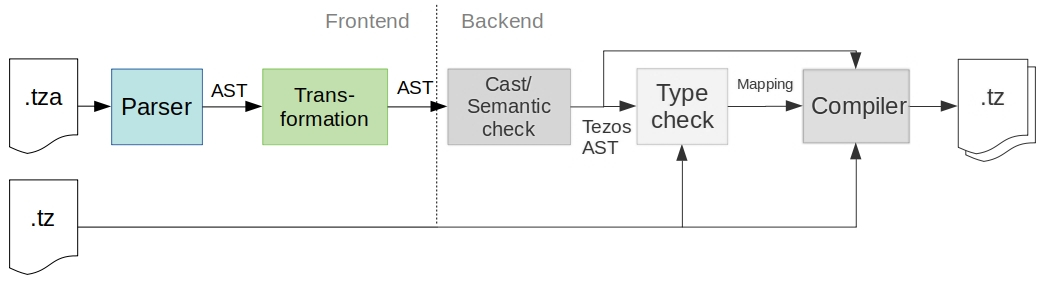
\includegraphics[width=\linewidth]{figures/3-offline/pipeline_frontend}
\caption{The stages of the generic frontend of the compilation pipeline}
\label{fig:pipeline_frontend}
\end{figure}

First, developers can specify assertions in a domain-specific language, which is described in \secref{sec:syntax}. The toolchain then parses the assertions into abstract syntax trees (ASTs), which are passed to the transformation stage. In this stage, the ASTs are transformed into ASTs that represent their negation. This is described further in \secref{sec:transformation}. The resulting ASTs are then passed to the backend, which is introduced in the \chapref{chap:offline_tezos} for the Tezos blockchain.

\section{Assertion Syntax}\label{sec:syntax}
Tezos' smart contract language Michelson is a low-level and stack-based language. Specifying assertions in such a target-specific language is complex and inconvenient, especially if the language should be compiled to other targets as well. Therefore, this thesis defines a domain-specific high-level language to express assertions. 

The syntax of this language is described in two versions by the grammars given in appendix \ref{apx:grammar}. One version implements a prefix and the other an infix notation. The parser currently supports the prefix notation and correct operator precedences must be handled explicitly with parentheses. To avoid context switches (for developers on Tezos), the syntax is inspired by OCaml and uses the same type notations as Michelson.

\subsection{Code Structure}
Assertions are passed to the toolchain as simple text files. This thesis follows the convention of using the file extension \texttt{.tza} for such files (henceforth referred to as ``assertion contracts''), in reference to the file extension \texttt{.tz} used for Michelson source files. An assertion contract is always associated with a smart contract (henceforth referred to as ``parent contract'') and contains at least one assertion for a specific entrypoint thereof. For the remaining entrypoints, the compiler should automatically generate empty assertions (cf. \secref{sec:compiler}).

An assertion begins with the keyword \texttt{entrypoint} and a signature consisting of an optional tag, denoted by \%, followed by a parameter pattern. Parameter patterns are similar to patterns in OCaml --- they are templates that match shapes of data structures and bind identifiers to the components of them. The given parameter pattern must match exactly the parameter type of the entrypoint it is associated with. The body of an assertion can contain a nesting of quantifiers and conditions around exactly one \texttt{assert} expression, which tests a property. Conditions can be used to restrict the quantification domains or to impose any other constraints. For completeness, the existential quantifier is already included in the grammar, however the current version of the pipeline will reject any assertions containing it. 

How the assertions are associated with the respective entrypoint of the parent contract, may depend on the smart contract language. In the case of Solidity, a tag that mirrors the function name is enough to link assertion and entrypoint. In Michelson contracts, on the other hand, entrypoints can be anonymous. Therefore, the assertions are linked to the entrypoints through the tags, the parameter type or both. How the linking is implemented in the Tezos backend is described in more detail in \secref{sec:typecheck}.

\subsection{Parameter Patterns}
\lstref{lst:patterns} gives an overview of the parameter patterns supported in the assertion language.
\lstinputlisting[caption=Patterns in the assertion language, language=, numbers=none, label=lst:patterns]{listings/patterns.txt}
By using patterns, developers can avoid the explicit handling of special cases, such as empty lists, in the assertion specification. Furthermore, they can be used to put emphasis on the relevant components of the input parameters by replacing the irrelevant ones with wildcards. As an example, the assertion given in \lstref{lst:patterns_usage} concerns the left element of a pair and only applies to non-empty lists. 
\begin{lstlisting}[label=lst:patterns_usage, language=Assertion, numbers=none]
(entrypoint %g (pair (cons a as) _)  ...)
\end{lstlisting}

\subsection{Types and Operations}
In order to make the frontend generic, the sets of data types and operations supported by the grammar constitute unions of those present in the target languages. This allows not only the implementation of a single, common parser, but also the transformation to be oblivious of the target platform. As a consequence, the backends are responsible for performing a semantic check and  rejecting any assertions containing types or operations which are not supported by the target language.

The current version of the language contains all data types present in Tezos' VM and a subset of operations that Michelson provides (as of protocol version 007 Delphi). Besides the primitive types \texttt{int}, \texttt{nat} (natural numbers), \texttt{string}, \texttt{bool}, \texttt{bytes} and \texttt{unit}, this includes composite types like \texttt{list}, \texttt{pair}, \texttt{map} or the union type \texttt{or}. Domain specific data types, like \texttt{timestamp} or \texttt{address}, are supported as well. The data type \texttt{fmu} represents a generic fractional monetary unit, which is translated to the corresponding token type of the target platform\footnote{For example Mutez in Tezos, or Wei in Ethereum}.

The grammar currently includes common arithmetic (e.g., \texttt{add}, \texttt{sub}, \texttt{abs}, \texttt{mod}), relational  (e.g., \texttt{eq}, \texttt{neq}, \texttt{lt}) and logic and bitwise operators (e.g., \texttt{and}, \texttt{or}, \texttt{lsr}, \texttt{lsl}). Some operations that operate on data structures (e.g., \texttt{nth} and \texttt{size}) are supported as well. Domain specific operations have not been included yet, but they may be added to the language if necessary. \\

Let us consider a variation of the explicit assertion for sorted lists, stated in \eqref{eq:sorted_v2}. In contrast to the variation given in the introduction (\eqref{eq:sorted}), which translates to comparing a random element of the list with its direct neighbour, this translates to a comparison of two random elements (under the constraint $n < m$). \lstref{lst:sorted_assertion} shows how this formula can be expressed in the assertion language.
\begin{equation}\label{eq:sorted_v2}
	(\forall n,m : int) (0 \leq n < m < |a|) \Rightarrow a[n] \leq a[m]
\end{equation}
\lstinputlisting[caption=Assertion specification for sorted lists, language=Assertion, label={lst:sorted_assertion}]{listings/sorted.tza}

Line 1 declares the signature of the assertion. It specifies the explicit tag \textit{find} and the input parameter \texttt{a} of type integer list. The body is a nesting of two universal quantifiers, which declare the predicate variables $n$ and $m$ of type integer (lines 2 and 3), followed by a nesting of conditions. The conditions define the domains of the quantifiers (lines 4-7), corresponding to the premise of the formula. The body of the last condition (line 7) ultimately contains the keyword \texttt{assert} followed by a condition checking the property of ascending order, i.e.,  $a[n] \leq a[m]$.

\subsection{Extensions}\label{sec:ext}
In future iterations, the assertion syntax could be extended with some more features to improve usability and readability:
\begin{itemize}
\item \textbf{Local variables} to store, reuse and denominate computed values
\item \textbf{User-defined functions} to extract whole routines, s.t. they can be reused in several assertions or other assertion contracts
\item \textbf{if-else conditions} to adapt the domains of quantifications if certain conditions hold. The assertion checking whether two numbers are relatively prime (introduced in \secref{sec:coprime}) is a good use-case for this feature: firstly, the formula requires to determine the minimum of the given numbers --- however, the \texttt{min}-function might not be supported as a built-in function by the target language (as is the case in Michelson). A solution for that is to implement two branches in the program to handle each case. Secondly, if the greater of the two numbers is not evenly divided by the smaller one, the formula can be optimized by reducing the quantification domain by half to $2 \le n \le \lfloor \frac{min(a,b)}{2} \rfloor$. \lstref{lst:coprime} shows a hypothetical specification of an assertion validating the property of coprimeness using \texttt{if-else} control structures:
\lstinputlisting[caption=Assertion for coprimeness using if-else structures, language=Assertion, label={lst:coprime}]{listings/coprime_ifelse.tza}
\end{itemize}

\section{Parser}
Assertions expressed in the syntax described above are passed as a simple text file to the pipeline. It is not admissible to generate empty assertions for all entrypoints of the parent contract, hence empty files are rejected. Furthermore, the parser guarantees total success or total failure of parsing the assertion by aborting execution immediately after encountering a syntax error. 

After successfully parsing all assertions, the parser returns a list of their corresponding ASTs. \lstref{lst:ast_type} shows the toplevel definition of the AST type in OCaml. It is composed of an entrypoint specification, consisting of an optional tag and the parameter pattern, and an assertion body. The parameter pattern and assertion body are subtrees representing their composition, or the nested assertion code respectively.
\begin{lstlisting}[label=lst:ast_type, language=, numbers=none, caption=Toplevel AST type definition in OCaml]
type ast =
  {entrypoint : string option * pattern; body : assertion}
\end{lstlisting}

\figref{fig:ast_example} shows the resulting AST after parsing the assertion given in \lstref{lst:sorted_assertion}. The subtype representing quantifiers contains a special field \textit{Bounds}, which is initially left empty by the parser. During the transformation, it is populated with a set of constraints concerning its predicate variable. This is described in the following section.

\section{Transformation}\label{sec:transformation}
The assertion, as specified by a developer, is modified in two ways before the compiler translates it into target code: firstly, it has to be transformed into its negation. Secondly, quantifiers are converted to random generators, which generate values within a specified range (corresponding to the domains of discourse). In the assertion language, the ranges can be expressed using \texttt{if}-conditions. As a preliminary for the compilation, the transformation thus analyses the condition nodes of the AST, identifies conditions that state a range constraint for a generator and assigns it to the respective quantification node (by adding it to the \textit{Bounds} field). Therefore, the transformation contains two consecutive steps:
\begin{enumerate}
\itemsep-0.5em
\item Negation
\item Domain constraint analysis and assignment
\end{enumerate}
Each step is described in more detail in the following subsections.

\subsection{Negation}
The formula is negated according to the negation rules of second-order predicate logic and by applying De Morgan's laws \cite{de_morgan} until the negation is applied to the literals. Negating universal quantification is equivalent to an existential quantification of its negated body (and vice versa): $\neg \forall x P(x) \equiv \exists x \neg P(x)$ \cite{Sundstrom2020Quantifiers}. The domain restrictions are not affected by the negation. This is also reflected in the negation rules of predicate logic, if the domain is given as an implication premise in the logical formula: $\neg (p \Rightarrow q) \equiv p \Rightarrow \neg q $. 

Applied to an AST representation of the assertion, the negation recursively traverses the \texttt{assertion} subtree, replaces quantifier and expression nodes with the corresponding negations and skips condition nodes. Further pursuing the example of the assertion for sorted lists, the negated version of the AST given in \figref{fig:ast_example} is shown in \figref{fig:ast_example_neg}. The universal quantifiers have been transformed to existential quantifiers, and the subtree of \texttt{assert}, representing the property check $a[n] <= a[m]$, to the negated expression $a[n] > a[m]$.

\begin{figure}[t]
\hfill
\subfloat[AST after parsing\label{fig:ast_example}]{%
  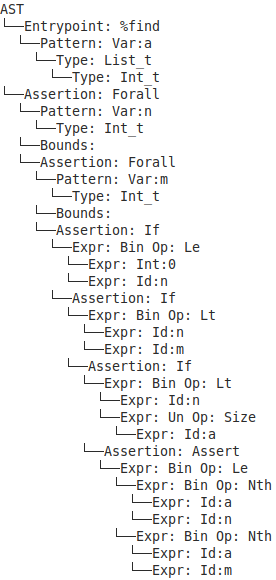
\includegraphics[width=0.33\textwidth]{figures/3-offline/ast_example_find}
}
\subfloat[Negated AST\label{fig:ast_example_neg}]{%
  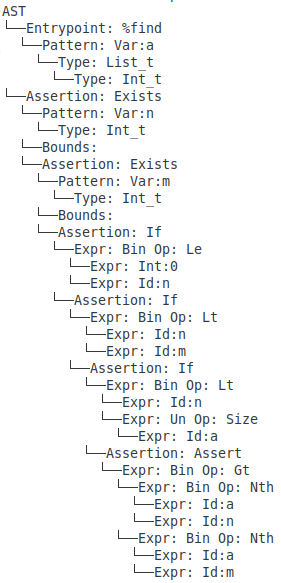
\includegraphics[width=0.33\textwidth]{figures/3-offline/ast_example_neg}
}
\hfill
\subfloat[Fully transformed AST\label{fig:ast_example_transf}]{%
  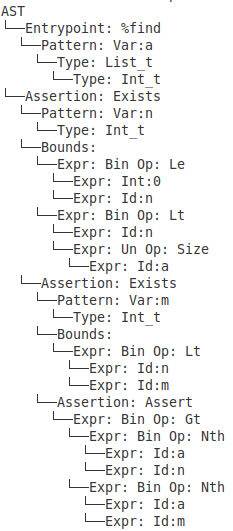
\includegraphics[width=0.3\textwidth]{figures/3-offline/ast_example_transf}
}
\caption{Modifications to the sorted list assertion AST from parsing to completed transformation}
\end{figure}

\subsection{Domain Assignment}\label{sec:transf_domains}
In order to obtain random generators which only generate values in the interesting range, i.e., within the domains of discourse, the second step of the transformation skims the condition nodes of the AST for atomic constraints containing bound variables. These conditions are then moved to the \texttt{Bounds} field of the respective quantifier binding that variable. If the constraint contains more than one bound variable, it is assigned to the quantifier with the highest depth in the quantifier nesting. When translating the quantifiers to random generators, their ranges can then be constructed based on the associated list of constraints. After merging a constraint with a quantifier node, it is removed from the assertion body, as checking these constraints during runtime becomes redundant. Constraints not involving bound variables have to be checked during runtime. 

The assertion for sorted lists contains the four constraints
\begin{enumerate}
\itemsep-1em
\item $0 \leq n$
\item $n < |a| $
\item $n \le m$ and
\item $m < |a|$.
\end{enumerate}
Constraint 1,2 and 4 only contain one bound variable ($n$ or $m$), hence they are assigned to the respective quantifier binding it. Constraint 3 features two bound variables -- this constraint is assigned to the quantifier furthest in the nesting, i.e., the quantifier binding $m$. The corresponding AST expressing this assignment is shown in \figref{fig:ast_example_transf}. Based on the assigned constraints, the compiler can then translate the quantifiers to the random generators as indicated in \lstref{lst:rand}.
\begin{lstlisting}[label=lst:rand, caption=Random generators for the sorted list assertion, numbers=none]
n = random(0, size(a))
m = random(n + 1, size(a))
\end{lstlisting}

For constraints containing certain operators, deriving efficient random generators is less straight-forward. Consider the following constraints:
\begin{enumerate}
\itemsep-0.7em
\item $(\forall n : int) (n < 10 \lor n > 20) ...$
\item $(\forall n,m : int) (n < 10 \lor m > 20)$
\item $(\forall n : int) (n \ne 10) ...$
\item $(\forall n : int) (n = 10) ...$
\end{enumerate}
Constraint 1 separates the range into two disjoint sub-ranges, which translates to a random generator as shown in \lstref{lst:rand_disjoint}.
\begin{lstlisting}[label=lst:rand_disjoint, caption=Random generator with two disjoint ranges, numbers=none]
n = if random(0,2) == 0 then random(-MAX_INT, 10)
                        else random(21, MAX_INT)
\end{lstlisting}
If a disjunction involves several bound variables, as in constraint 2, the operands of this disjunction cannot be considered separately, as would be the case with a conjunction. For the predicate variable whose random generator is executed first, the domain restriction is optional, while the generation of the following random value depends on the previous result. \lstref{lst:rand_disjoint_nm} shows the corresponding random generators for this case.
\begin{lstlisting}[label=lst:rand_disjoint_nm, caption=Random generators of a disjunction of constraints with two bound variables, numbers=none]
n = if random(0,2) == 0 then random(-MAX_INT, 10)
                        else random(-MAX_INT, MAX_INT)
m = if n < 10 then random(-MAX_INT, MAX_INT)
              else random(20, MAX_INT)
\end{lstlisting}
Similarly to 1, constraint 3 splits the domain into sub-domains. Constraint 4 effectively makes the quantifier binding $n$ obsolete and can therefore be translated to a constant value.

In the current implementation of the transformation, constraints featuring the logical or, exclusive or inequality operator are kept as part of the assertion body. They are considered to be exceptional cases, but will increase the overall complexity of the compilation beyond the scope of a first iteration. Constraints remaining within the assertion body will be checked during runtime. As a consequence, an invocation of the assertion contract can result in a futile assertion check if such a condition is not met.

\subsubsection{Implicit Constraints}
In some cases, boundaries are imposed to the random generators implicitly by the used data types. List indices, for instance, are always bound to the range $[0.. size(list))$ and could thus be derived from the formula without an explicit specification. As this requires a semantic analysis of the AST and thus a more complex transformation, the current implementation requires a completely explicit formula in terms of the domains. 

Depending on the blockchain VM, the lower bound for generated values used in indexing operations can be implicitly handled by the random generator of an appropriate predicate variable type. As an example, Michelson supports the data type \texttt{nat} representing the natural numbers, which categorically excludes all values below zero. \eqref{eq:sorted_v2} can thus be abbreviated with the formula given in \eqref{eq:sorted_v2_abbr}.
\begin{equation}\label{eq:sorted_v2_abbr}
	(\forall n : nat)(\forall m : nat) (n \le m < |a|) \Rightarrow a[n] \leq a[m]
\end{equation}